\documentclass[11pt,class=report,crop=false]{standalone}
\usepackage{exo7sv}

\begin{document}

%%%%%%%%%%%%%%%%%%%%%%%%%%%%%%%%%%%%%%%%%%%%%%%%%%%%%%%%%%%%%%%%%%%%%%
%%%%%%%%%%%%%%%%%%%%%%%%%%%%%%%%%%%%%%%%%%%%%%%%%%%%%%%%%%%%%%%%%%%%%%

\entete{Université de Lille}{Mathématiques -- svte - 2020}

\titre{Fiche 11. \quad Longueur, aire, volume} 

\encadre{
	\emph{Savoir.}
	\begin{itemize}[label=$\square$]
		\item Connaître le lien entre intégrale et aire sous la courbe.

	\end{itemize}
	\emph{Savoir-faire.}
	\begin{itemize}[label=$\square$]
		\item Savoir appliquer les formules données pour calculer des longueurs, des aires et des volumes.
	\end{itemize}
}

\insertvideo{3Oa3Je_5NLg}{Fiche 11. Longueur, aire, volume}

\bigskip

Nous allons donner quelques exemples d'application du calcul intégral aux calculs d'aires, de longueurs ou de volumes.

%%%%%%%%%%%%%%%%%%%%%%%%%%%%%%%%%%%%%%%%%%%%%%%%%%%%%%%%%%%%%%%%%%%%%%
\subsection*{Aire sous une courbe}

On sait déjà que l'aire sous le graphe d'une fonction est mesurée par une intégrale.

\begin{minipage}{0.45\textwidth}
$$\mathcal{A} = \int_a^b f(x)\,\dd x$$
\end{minipage}
\begin{minipage}{0.5\textwidth}
\shorthandoff{?;:!}
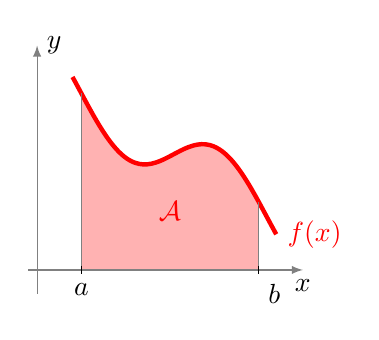
\begin{tikzpicture}[scale=1.5,xscale=1.5]
\tikzset{
	declare function={
		qcq(\t) = 1.5 - \t - 0.3*sin(6*(\t+1.05) r);
	}
}

 % tracé de la courbe et des axes
  \fill[red!30] (0,0) -- plot[domain=0:1] (\x,{qcq(\x)}) -- (1,0) -- cycle;
  \draw[ultra thick, color=red,domain=-0.05:1.1, smooth, samples=50] plot (\x,{qcq(\x)}) node[right] {$f(x)$};
  \draw[gray,->,>=latex] (-0.30,0) -- (1.25,0) node[below,black] {$x$};
  \draw[gray,->,>=latex] (-0.25,-0.2) -- (-0.25,1.9) node[right,black] {$y$};

  % tracé de la courbe par-dessus les rectangles
  % \draw[ultra thick, color=red,domain=-0.05:1.1, samples=100] plot (\x,{qcq(\x)}) node[right] {$y=f(x)$};
   \pgfmathparse{qcq(0)}   \let\y\pgfmathresult
   \draw[gray] (0,0) -- (0,\y);
   \pgfmathparse{qcq(1)}   \let\y\pgfmathresult
   \draw[gray] (1,0) -- (1,\y);

% du texte
  \draw (0 cm,1pt) -- (0 cm,-1pt) node[below] {$a$};
  \draw (1 cm,1pt) -- (1 cm,-1pt) node[below right] {$b$};
  \draw (0.5,0.5) node[color=red]{$\mathcal{A}$};
\end{tikzpicture}
\shorthandoff{?;:!}
\end{minipage}

\medskip

Cette propriété permet de calculer des aires délimitées par deux courbes.

\medskip

\begin{minipage}{0.4\textwidth}
\textbf{Exercice.}
Combien vaut l'aire représentée sur ce dessin ?
\end{minipage}\qquad
\begin{minipage}{0.45\textwidth}
	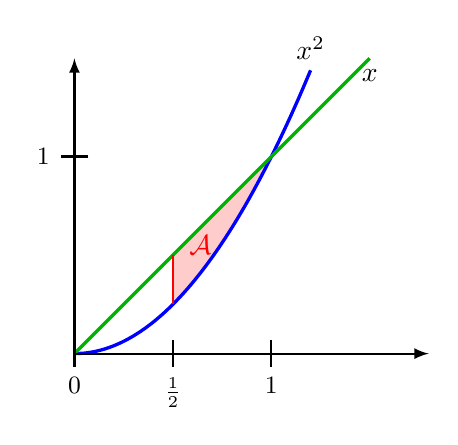
\begin{tikzpicture}
	\begin{scope}[scale=2.5]
	\filldraw[draw=red!20,fill=red!20]plot [smooth,domain=0.5:1] (\x,\x)-- plot [smooth,domain=1:0.5] (\x,\x^2)-- cycle;
	\draw[very thick,  domain=0:1.2, smooth,color=blue]plot(\x,{\x^2}) node[above,black]{$x^2$};
	\draw[very thick,  domain=0:1.5, smooth,color=green!70!black]plot(\x,\x) node[below,black]{$x$};
	\draw[color=red,thick] (0.5,0.25) -- (0.5,0.5);
	% \draw[color=red,dashed] (0.5,0.25) -- (0.5,0);
	\draw[thick,->,>=latex] (0,0)--(1.8,0); %node[above] {$x$};
	\draw[thick] (0,2pt) -- (0,-2pt)node[below] {\small$0$};
	\draw[thick] (1,2pt) -- (1,-2pt)node[below] {\small$1$};
	\draw[thick] (0.5,2pt) -- (0.5,-2pt)node[below] {\small$\frac{1}{2}$};
	\draw[thick,->,>=latex] (0,0)--(0,1.5); %node[above] {$y$};
	\draw[very thick] (2pt,1) -- (-2pt,1)node[left] {\small$1$};
	\draw (0.64,0.55) node[color=red]{$\mathcal{A}$};
	\end{scope}
	\end{tikzpicture}
\end{minipage}

\textbf{Solution.}
On note $f(x)=x$ et $g(x)=x^2$. 
L'aire $\mathcal{A}$ est délimitée par les graphes de la fonction $f$ et $g$, la droite d'équation $x=\frac{1}{2}$ (et la droite d'équation $x=1$).

Cette aire se calcule comme la différence des deux aires $\mathcal{A}_f - \mathcal{A}_g$.

\begin{center}
	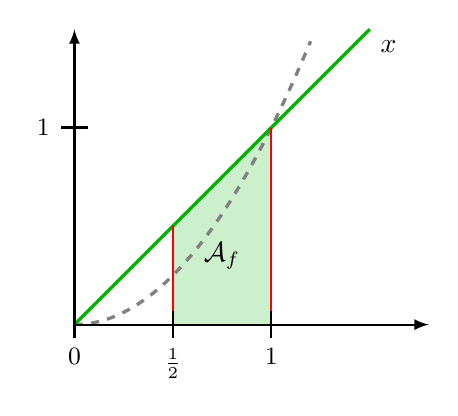
\begin{tikzpicture}
	\begin{scope}[scale=2.5]

	\fill[fill=green!70!black!20]plot [smooth,domain=0.5:1] (1,0) --  plot [smooth,domain=1:0.5] (\x,\x)-- (0.5,0)-- cycle;
	\draw[very thick, dashed, domain=0:1.2, smooth,color=gray]plot(\x,{\x^2});

	\draw[very thick,  domain=0:1.5, smooth,color=green!70!black]plot(\x,\x) node[below right,black]{$x$};
	\draw[color=red,thick] (0.5,0.5) -- (0.5,0);
	\draw[color=red,thick] (1,1) -- (1,0);
	% \draw[color=red,dashed] (0.5,0.25) -- (0.5,0);
	\draw[thick,->,>=latex] (0,0)--(1.8,0); %node[above] {$x$};
	\draw[thick] (0,2pt) -- (0,-2pt)node[below] {\small$0$};
	\draw[thick] (1,2pt) -- (1,-2pt)node[below] {\small$1$};
	\draw[thick] (0.5,2pt) -- (0.5,-2pt)node[below] {\small$\frac{1}{2}$};
	\draw[thick,->,>=latex] (0,0)--(0,1.5); %node[above] {$y$};
	\draw[very thick] (2pt,1) -- (-2pt,1)node[left] {\small$1$};
	\draw (0.75,0.35) node{$\mathcal{A}_f$};
	\end{scope}
	\end{tikzpicture}
\qquad\qquad
	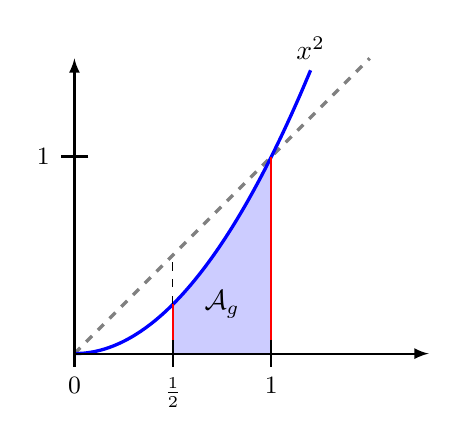
\begin{tikzpicture}
	\begin{scope}[scale=2.5]

	\fill[fill=blue!20](1,0) --  plot [smooth,domain=1:0.5] (\x,\x^2) -- (0.5,0) -- cycle;
	\draw[very thick, dashed,   domain=0:1.5, smooth,color=gray]plot(\x,\x);
	\draw[very thick, domain=0:1.2, smooth,color=blue]plot(\x,{\x^2}) node[above,black]{$x^2$};
	\draw[dashed] (0.5,0) -- (0.5,0.5);
	\draw[color=red,thick] (0.5,0) -- (0.5,0.25);
	\draw[color=red,thick] (1,0) -- (1,1);
	\draw[thick,->,>=latex] (0,0)--(1.8,0); %node[above] {$x$};
	\draw[thick] (0,2pt) -- (0,-2pt)node[below] {\small$0$};
	\draw[thick] (1,2pt) -- (1,-2pt)node[below] {\small$1$};
	\draw[thick] (0.5,2pt) -- (0.5,-2pt)node[below] {\small$\frac{1}{2}$};
	\draw[thick,->,>=latex] (0,0)--(0,1.5); %node[above] {$y$};
	\draw[very thick] (2pt,1) -- (-2pt,1)node[left] {\small$1$};
	\draw (0.75,0.25) node{$\mathcal{A}_g$};
	\end{scope}
	\end{tikzpicture}
\end{center}


On a donc:
\begin{align*}
\mathcal{A}
  &= \mathcal{A}_f - \mathcal{A}_g 
  = \int_{\frac{1}{2}}^{1}f(x) \, \dd x - \int_{\frac{1}{2}}^{1} g(x) \, \dd x \\
  &= \int_{\frac{1}{2}}^{1} f(x)-g(x)\,\dd x 
  = \int_{\frac{1}{2}}^{1}x-x^2 \,\dd x \\
  &= \bigg[\frac{x^2}{2}-\frac{x^3}{3}\bigg]_{\frac{1}{2}}^{1}  
  = \bigg(\frac{1}{2}-\frac{1}{3}\bigg)-\bigg(\frac{1}{8}-\frac{1}{24}\bigg) \\
  &= \frac{1}{12}.
\end{align*}

\subsection*{Longueur d'une courbe}

\textbf{Formule.}
Soit $f : [a,b] \to \Rr$ une fonction dérivable.
La longueur $\mathcal{L}$ de la courbe de $f$ entre les abscisses $a$ et $b$ est donnée par:

\begin{minipage}{0.45\textwidth}
\mybox{$\displaystyle \mathcal{L} = \int_{a}^{b} \sqrt{1+f'(x)^2} \, \dd x$}
\end{minipage}
\qquad
\begin{minipage}{0.5\textwidth}
\shorthandoff{?;:!}
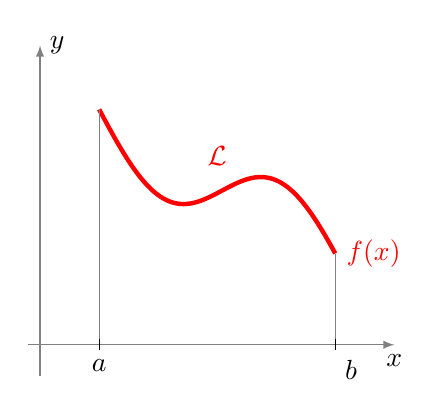
\begin{tikzpicture}[scale=2,xscale=1.5]
\tikzset{
	declare function={
		qcq(\t) = 1.5 - \t - 0.3*sin(6*(\t+1.05) r);
	}
}

 % tracé de la courbe et des axes
%  \fill[red!30] (0,0) -- plot[domain=0:1] (\x,{qcq(\x)}) -- (1,0) -- cycle;
  \draw[ultra thick, color=red,domain=0:1, smooth, samples=50] plot (\x,{qcq(\x)}) node[right] {$f(x)$};
  \draw[gray,->,>=latex] (-0.30,0) -- (1.25,0) node[below,black] {$x$};
  \draw[gray,->,>=latex] (-0.25,-0.2) -- (-0.25,1.9) node[right,black] {$y$};

   \pgfmathparse{qcq(0)}   \let\y\pgfmathresult
   \draw[gray] (0,0) -- (0,\y);
   \pgfmathparse{qcq(1)}   \let\y\pgfmathresult
   \draw[gray] (1,0) -- (1,\y);

% du texte
  \draw (0 cm,1pt) -- (0 cm,-1pt) node[below] {$a$};
  \draw (1 cm,1pt) -- (1 cm,-1pt) node[below right] {$b$};
  \draw (0.5,1.2) node[color=red]{$\mathcal{L}$};
\end{tikzpicture}
\shorthandoff{?;:!}
\end{minipage}

\bigskip

\emph{Cette formule n'est pas à connaître, elle sera donnée à chaque fois, mais il faut savoir l'appliquer !}

\bigskip

\begin{minipage}{0.5\textwidth}
\textbf{Exercice.}
Quelle est la longueur de cette portion de courbe définie par $f(x) = \frac23(x-1)^{\frac32}$ sur l'intervalle $[1,4]$ ?
\end{minipage}\qquad
\begin{minipage}{0.45\textwidth}
	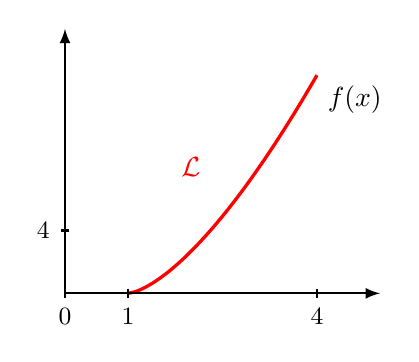
\begin{tikzpicture}
	\begin{scope}[scale=0.8]
	\draw[very thick,  domain=1:4, smooth,color=red]plot({\x},{2/3*(\x-1)^(3/2)}) node[below right,black]{$f(x)$};
%	\draw[color=red,thick] (0.5,0.25) -- (0.5,0.5);
	% \draw[color=red,dashed] (0.5,0.25) -- (0.5,0);
	\draw[thick,->,>=latex] (0,0)--(5,0); %node[above] {$x$};
	\draw[thick] (0,2pt) -- (0,-2pt)node[below] {\small$0$};
	\draw[thick] (1,2pt) -- (1,-2pt)node[below] {\small$1$};
	\draw[thick] (4,2pt) -- (4,-2pt)node[below] {\small$4$};
%	\draw[thick] (0.5,2pt) -- (0.5,-2pt)node[below] {\small$\frac{1}{2}$};
	\draw[thick,->,>=latex] (0,0)--(0,4.2); %node[above] {$y$};
	\draw[very thick] (2pt,1) -- (-2pt,1)node[left] {\small$4$};
	\draw (2,2) node[color=red]{$\mathcal{L}$};
	\end{scope}
	\end{tikzpicture}
\end{minipage}


\bigskip

\textbf{Solution.}
%On rappelle que $u^{\frac32} = u \sqrt{u}$ et que sa dérivée est $\frac32 u' u^{\frac12} = \frac32 u' \sqrt{u}$.

Considérons $f(x) = \frac23(x-1)^{\frac32}$ sur l'intervalle $[1,4]$.
Alors $f'(x) = \sqrt{x-1}$, donc $f'(x)^2 = x-1$.
Ainsi :
\begin{align*}
\mathcal{L} 
  &= \int_1^4 \sqrt{1+f'(x)^2} \, \dd x
  = \int_1^4 \sqrt{1+\sqrt{x-1}^2} \, \dd x \\
  &= \int_1^4 \sqrt{1+(x-1)} \, \dd x 
  = \int_1^4 \sqrt{x} \, \dd x \\
  &= \bigg[ \frac23 x^{\frac32} \bigg]_{1}^{4} 
  = \frac23(8-1) = \frac{14}{3}. \\
\end{align*}

\subsection*{Volume}


\textbf{Formule.}
Soit $f : [a,b] \to \Rr$ une fonction. On considère l'objet obtenu par rotation du graphe de $f$ autour de l'axe des abscisses. Le volume $\mathcal{V}$ de l'objet est donné par:
\mybox{$\displaystyle \mathcal{V}=\int_{a}^{b}\pi f(x)^2 \, \dd x$}

\emph{Cette formule n'est pas à connaître.}

\bigskip

\begin{minipage}{0.35\textwidth}
\textbf{Exercice.}
Quel volume est obtenu par rotation du graphe de
$f(x)=\frac{x}{2}$ autour de l'axe des abscisses 
sur l'intervalle $[0,4]$ ?
\end{minipage}
\quad
\begin{minipage}{0.33\textwidth}
	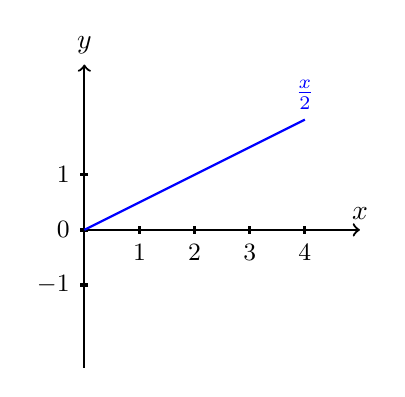
\begin{tikzpicture}
	\begin{scope}[yscale=0.7,xscale=0.7]
	\draw[thick,->] (0,0)--(5,0)node[above] {$x$};
	\foreach\x in{1,...,4}{\draw[very thick] (\x,2pt) -- (\x,-2pt)node[below] {\small$\x$};}
	\draw[thick,->] (0,-2.5)--(0,3)node[above] {$y$};
	\foreach\y in{-1,...,1} {\draw[very thick] (2pt,\y) -- (-2pt,\y)node[left] {\small$\y$};}
	\draw[ thick,  domain=0:4, smooth,color=blue]plot(\x,\x/2) node[above]{$\frac{x}{2}$};
    \end{scope}
\end{tikzpicture}
\end{minipage}
\begin{minipage}{0.4\textwidth}
	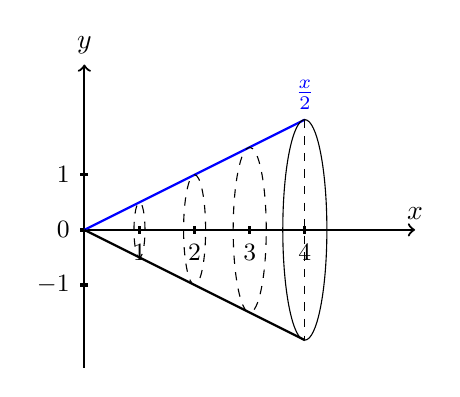
\begin{tikzpicture}
	\begin{scope}[yscale=0.7,xscale=0.7]
	\draw[thick,->] (0,0)--(6,0)node[above] {$x$};
	\foreach\x in{1,...,4}{\draw[very thick] (\x,2pt) -- (\x,-2pt)node[below] {\small$\x$};}
	\draw[thick,->] (0,-2.5)--(0,3)node[above] {$y$};
	\foreach\y in{-1,...,1} {\draw[very thick] (2pt,\y) -- (-2pt,\y)node[left] {\small$\y$};}
	\draw[ thick,  domain=0:4, smooth,color=blue]plot(\x,\x/2) node[above]{$\frac{x}{2}$};
	\draw[ thick,  domain=0:4, smooth,color=black]plot(\x,-\x/2);
	\draw[color=black] (4,0) circle (0.4cm and 2cm);
	\draw[color=black,dashed] (3,0) circle (0.3cm and 1.5cm);
	\draw[color=black,dashed] (2,0) circle (0.2cm and 1cm);
	\draw[color=black,dashed] (1,0) circle (0.1cm and 0.5cm);
	\draw[dashed] (4,2) -- (4,-2);
    \end{scope}
\end{tikzpicture}
\end{minipage}

\bigskip

\textbf{Solution.}
Soit $f : [0,4] \to \Rr$ définie par $f(x) = \frac{x}{2}$. 
Par rotation du graphe de $f$ autour de l'axe des abscisses, on obtient un cône ayant pour sommet l'origine.
La formule du volume s'écrit :
\[\mathcal{V}=\int_{0}^{4}\pi f(x)^2 \, \dd x=\pi\int_{0}^{4} \frac{x^2}{4} \,\dd x=\frac{\pi}{4}\bigg[\frac{x^3}{3}\bigg]_{0}^{4}=\frac{16\pi}{3}.\]

\emph{Exercice.} Retrouver ce résultat en appliquant la formule du volume d'un cône $\mathcal{V} = \frac13 S h$, ou $S$ est la surface de la base (ici l'aire du disque en $x=4$) et $h$ la hauteur (ici $h=4$).



\subsection*{Aire de la surface d'un objet}
\textbf{Formule.}
Soit $f : [a,b] \to \Rr$ une fonction positive. On considère l'objet obtenu par rotation du graphe de $f$ autour de l'axe des abscisses. L'aire $\mathcal{S}$ de la surface de l'objet obtenu est donnée par:
\mybox{$\displaystyle\mathcal{S}=\int_{a}^{b}2\pi f(x)\sqrt{1+f'(x)^2}\dd x.$}

\emph{Cette formule n'est pas à connaître.}

\bigskip

\begin{minipage}{0.35\textwidth}
	\textbf{Exercice.}
	Quelle est l'aire de la surface de l'objet obtenu par rotation du graphe de
	$f(x)=\frac{x}{2}$ autour de l'axe des abscisses 
	sur l'intervalle $[0,4]$ ?
\end{minipage}
\quad
\begin{minipage}{0.33\textwidth}
	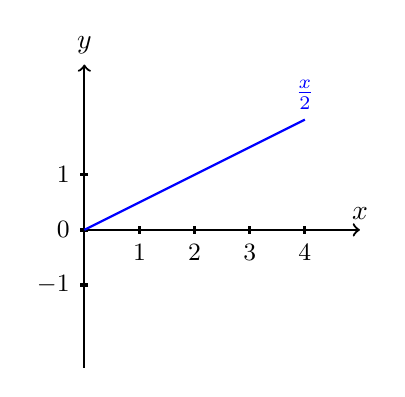
\begin{tikzpicture}
	\begin{scope}[yscale=0.7,xscale=0.7]
	\draw[thick,->] (0,0)--(5,0)node[above] {$x$};
	\foreach\x in{1,...,4}{\draw[very thick] (\x,2pt) -- (\x,-2pt)node[below] {\small$\x$};}
	\draw[thick,->] (0,-2.5)--(0,3)node[above] {$y$};
	\foreach\y in{-1,...,1} {\draw[very thick] (2pt,\y) -- (-2pt,\y)node[left] {\small$\y$};}
	\draw[ thick,  domain=0:4, smooth,color=blue]plot(\x,\x/2) node[above]{$\frac{x}{2}$};
	\end{scope}
	\end{tikzpicture}
\end{minipage}
\begin{minipage}{0.4\textwidth}
	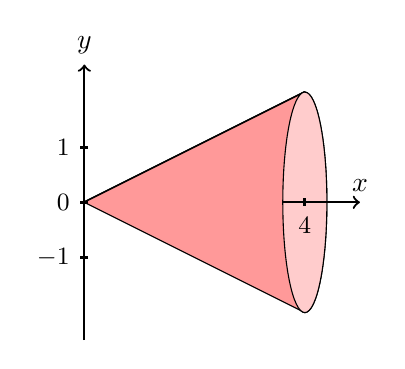
\begin{tikzpicture}
	\begin{scope}[yscale=0.7,xscale=0.7]
	\draw[ thick,  domain=0:4, smooth,color=black]plot(\x,\x/2);
	\draw[ thick,  domain=0:4, smooth,color=black]plot(\x,\x/2);
	\draw[color=black] (4,0) circle (0.4cm and 2cm);
	\draw [fill=red!40!white,opacity=1] (4,2) -- (4,-2) -- (0,0) -- cycle;
	\draw[color=black,fill=red!20!white,opacity=1] (4,0) circle (0.4cm and 2cm);
	\draw[thick,->] (3.6,0)--(5,0)node[above] {$x$ };
	\draw[very thick] (4,2pt) -- (4,-2pt)node[below] {\small$4$};
	\draw[thick,->] (0,-2.5)--(0,2.5)node[above] {$y$};
	\foreach\y in{-1,0,1} {\draw[very thick] (2pt,\y) -- (-2pt,\y)node[left] {\small$\y$};}
	\end{scope}
\end{tikzpicture}
\end{minipage}

\bigskip

\textbf{Solution.}
Soit $f : [0,4] \to \Rr$ définie par $f(x) = \frac{x}{2}$. 
Par rotation du graphe de $f$ autour de l'axe des abscisses, on obtient un cône ayant pour sommet l'origine.
La formule de la surface du cône s'écrit :
\[\mathcal{S}=\int_{0}^{4}2\pi f(x)\sqrt{1+f'(x)^2}\;\dd x
= 2\pi\int_{0}^{4} \frac{x}{2}\sqrt{1+\frac{1}{4}}\;\dd x 
= \frac{\pi\sqrt{5}}{2}\bigg[\frac{x^2}{2}\bigg]_{0}^{4}
= \frac{\pi\sqrt{5}}{2}\times \frac{4^2}{2}
= 4\pi\sqrt{5}.\]

\end{document}